\documentclass[11pt]{article}
\usepackage[latin1]{inputenc}
\usepackage[english]{babel}
\usepackage[centertags]{amsmath}
\usepackage{amsthm}
\usepackage{amssymb}
\usepackage[pdftex]{graphicx}
\usepackage{lastpage}
\usepackage{listings}
\usepackage{fancyhdr}
\usepackage[
	pdftex,
	pdfstartview={FitH},
	pdfstartpage=1,
	bookmarks=false,
	colorlinks=true,
	citecolor=black,
	linkcolor=black,
	urlcolor=black,
	pdfauthor=Svein~Baardsen
]{hyperref}


\newcommand{\name}{Svein~Baardsen}
\newcommand{\mail}{\href{mailto:sabaards@math.uio.no}{sabaards@math.uio.no}}
\newcommand{\course}{INF4490}
\newcommand{\project}{Mandatory assignment 1\\Travelling Salesman Problem}


\newcommand{\bigO}[1]{\mathcal{O}\left(#1\right)}

\renewcommand{\theequation}{\Roman{equation}}
\renewcommand{\thesubsection}{\arabic{subsection}.}

\fancypagestyle{plain}{%
\fancyhf{}%
\cfoot{Page \thepage\ of \pageref*{LastPage}}%
\renewcommand{\headrulewidth}{0pt}}%

\pagestyle{fancy}
\fancyhead{} \fancyfoot{}%
\lhead{\name} \chead{\course} \rhead{\today}%
\cfoot{Page \thepage\ av \pageref*{LastPage}}

\begin{document}
\lstset{language=Python,numbers=left,frame=single,tabsize=2}
\title{\course~- Biologically Inspired Computing\\\project}
\author{\name\\\mail}
\date{\today}
\maketitle \thispagestyle{plain} %\clearpage
\setlength{\parindent}{0pt}\setlength{\parskip}{11pt}%

\subsection*{Introduction}
My programme for the assignment is \textit{oblig1.py}. It takes one required parameter \textit{method} that can be one of the values: \textit{brute-force}, \textit{hill-climb}, \textit{ga} and \textit{hybrid}. In addition it can take the optional parameters \textit{cities} (number of cities), \textit{population} (population size), \textit{generations} (max number of generations), \textit{runs} (number of times the algorithm is run) and \textit{no-change} (number of generations without improvement before algorithm terminates). The programme requires python 3.6 to run.

\clearpage
\subsection{Exhaustive Search}
I start by running my implementation with a low number of cities: 
\[\textit{python oblig1.py --method brute-force --cities N}\] 
My programme then completes in the times shown below:

\begin{tabular}{l*{7}{|c}}
	Cities & 5 & 6 & 7 & 8 & 9 & 10 & 11\\
	\hline
	Time (s) & 0.000501 & 0.00100 & 0.00852 & 0.0732 & 0.685 & 7.54 & 86.9
\end{tabular}

For 10 cities I get that the shortest tour has length 7486.30999 and that one sequence that gives this length is: Hamburg, Brussels, Dublin, Barcelona, Belgrade, Istanbul, Bucharest, Budapest, Berlin and Copenhagen. 

Since the algorithm produces and checks all permutations of the cities I would expect the complexity to be \(\bigO{n!}\) and the time table above also seems to support this. A (very rough) estimate of the running time for 24 cities would then be:
\[T_{24}\approx T_{10}\frac{24!}{10!}\approx 1.3\cdot10^{18} seconds \approx 4\cdot10^{10} years\]
So we can safely conclude that an exhaustive search is not a feasible algorithm to use except for a very small number of cities.


\subsection{Hill Climbing}
I now run my programme with the parameters:
\[\textit{python oblig1.py --method hill-climb --cities N --no-change 100 --runs 20}\] 
The programme then runs the hill climbing algorithm with a random starting tour 20 times. The algorithm terminates when 100 generations in a row have failed to produce a better tour. The result for 10 and 24 cities can be seen in the following table:

\begin{tabular}{c*{5}{|c}}
	Cities & Time(s) & Worst & Mean & Best & \(\sigma\) \\
	\hline
	10 & 0.002 & 8407.18 & 7736.52 & 7486.31 & 373.619\\
	24 & 0.006 & 19184.42 & 16537.85 & 13718.49 & 1377.632
\end{tabular}

For 10 cities the algorithm has managed to find the global minimum im at least some of the runs, and it has done so in a fraction of the time it took the exhaustive search algorithm. 

When i run the programme with 24 cities the algorithm usually gives a different shortest length each time. I have also tried to increase the number of no-change generations before termination; increasing it to 1000 seems to give a better result without increasing the running time much but further increases did not seem to improve the result. And even for higher values the shortest length still changes for every run, it seems that we are past the limit of where hill climbing can reasonably be expected to find the best solution although it does find good solutions very fast.


\subsection{Genetic Algorithm}
For the genetic algorithm I have chosen to use inversion as the mutation operator and partially mapped crossover as the recombination operator. I chose these primarily because preservation of adjacency information is vital for TSP solvers but I have not had time to check whether some alternate operators would give better results.

For population initialization I use a purely random selection of tours, for parent selection I take the top 20\% of the population and pair them up randomly. To make sure that the algorithm will eventually terminate I have also set a limit of max 1000 generations but I have yet to see it reach this limit.

I start with a population of 100 and 10 cities. The algorithm then usually finds the optimal solution if it terminates after no change for 10 generations. With termination after 20 no-change generations I have yet to see it fail to find the optimal solution.

The table below is for 10 cities and termination after 20 generations without improvement:

\begin{tabular}{c*{5}{|c}}
	Population & Time(s) & Worst & Mean & Best & \(\sigma\) \\
	\hline
	10 & 0.003 & 8733.92 & 7962.72 & 7486.31 & 384.55\\
	100 & 0.029 & 7680.49 & 7514.08 & 7486.31 & 61.00\\
	1000 & 0.254 & 7603.24 & 7492.16 & 7486.31 & 25.48
\end{tabular}

We can tune the parameters a bit more because when we increase the population we can also decrease the number of no-change generations before termination. For population 1000 I can decrease no-change to 5 and the algorithm will still (almost always) find the optimal solution within 20 runs, this will also decrease the running time to 0.07 seconds. But still, for 10 cities I would say that a population of 10 is the better choice of the 3 because it does (usually) find the optimal solution very fast even if the standard deviation is pretty high.

The following table is for 24 cities and termination after 20 generations without improvement:

\begin{tabular}{c*{5}{|c}}
	Population & Time(s) & Worst & Mean & Best & \(\sigma\) \\
	\hline
	10 & 0.009 & 21350.85 & 17675.02 & 14764.20 & 1932.24\\
	100 & 0.092 & 18707.59 & 15584.73 & 13365.60 & 1686.27\\
	1000 & 0.868 & 18397.76 & 15414.86 & 13820.79 & 1080.67
\end{tabular}
\begin{figure}[!ht]
  \begin{center}
    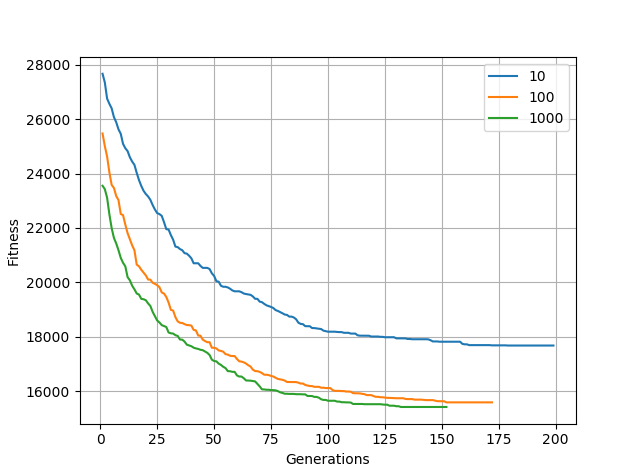
\includegraphics[width=.9\columnwidth]{ga3.png}
    \caption{Average length, over 20 runs, of tour of 24 cities per generation with different population sizes.}
  \end{center}
\end{figure}

From the table we can see that a population of 1000 is not that different from 100, and in the chart we can see that they reach about the same fitness with only 20 generations between them. And since 100 is so much faster I would say that it is the better of the two. For population 10 we see that it is significantly worse both in the table and the chart; we can of course improve this by increasing the number of no-change generations. But when I've tweaked the variables so they have about the same running time, I've found that population 100 is usually the more accurate of the two. And so a higher population of 100 seems to be preferable when the number of cities were increased.

The genetic algorithm will of course finish significantly faster than the exhaustive search and it seems to be about comparable to the hill climber. When I run it on 10 cities it on average inspects about 1200 tours. This is a lot less than the 10! = 3 628 800 that the exhaustive search inspects.

\subsection{Hybrid Algorithm}
With the hybrid algorithm I run the hill climber on every new child and stop after 5 generations without improvement. I've not had time to experiment a lot with this but 5 generations seemed to be a good compromise between speed and accuracy. 

The following table is for 24 cities and termination after 10 generations without improvement using a Lamarckian learning model:

\begin{tabular}{c*{5}{|c}}
	Population & Time(s) & Worst & Mean & Best & \(\sigma\) \\
	\hline
	10 & 0.012 & 20672.35 & 18073.84 & 14533.58 & 1599.46\\
	100 & 0.145 & 19072.81 & 16382.48 & 14155.39 & 1179.91\\
	1000 & 1.293 & 16964.07 & 15931.41 & 14053.76 & 702.41
\end{tabular}
\clearpage
\begin{figure}[!ht]
	\begin{center}
		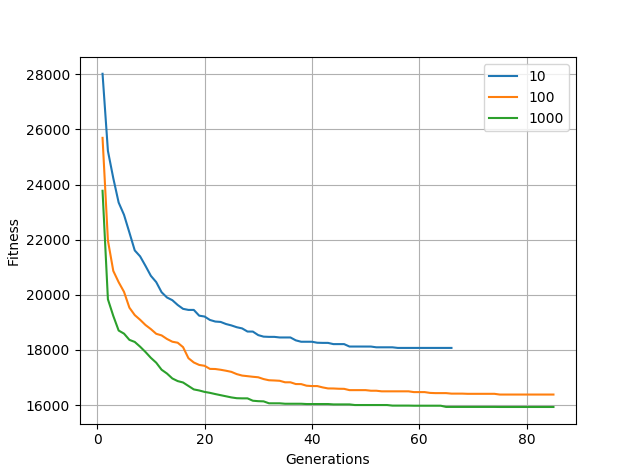
\includegraphics[width=.9\columnwidth]{hy3.png}
		\caption{Average length, over 20 runs, of tour of 24 cities per generation with different population sizes.}
	\end{center}
\end{figure}

I chose to stop after 10 generations because that gave running times that were fairly comparable to the genetic algorithm. When we compare the tables we see that the only advantage the hybrid algorithm has over the GA is a lower standard deviation. In the chart we can see that the hybrid algorithm terminates after less than half of the generations that the GA used. I've also found that the hybrid algorithm inspects about 4-5 times as many tours as the GA when the tours inspected by the hill climber is included. I've not been able to find any way to tweak the hybrid algorithm to make it better compared with the GA.

When using a Baldwinian learning model we get the table and chart on the next page. I haven't been able to tweak the model to give it any advantage over the Lamarckian. It either takes a longer time or it has a lower accuracy, and sometimes both.

\begin{tabular}{c*{5}{|c}}
	Population & Time(s) & Worst & Mean & Best & \(\sigma\) \\
	\hline
	10 & 0.011 & 23853.10 & 21430.41 & 19610.40 & 970.51\\
	100 & 0.112 & 20492.62 & 19293.02 & 18243.62 & 545.76\\
	1000 & 1.224 & 18884.26 & 18111.01 & 16679.77 & 660.76
\end{tabular}
\begin{figure}[!ht]
	\begin{center}
		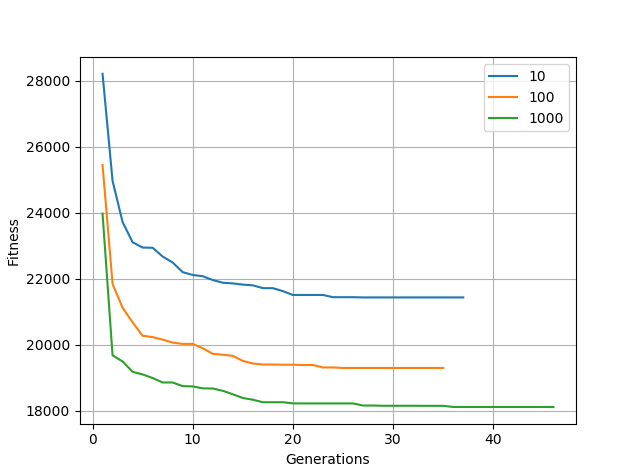
\includegraphics[width=.9\columnwidth]{hb3.png}
		\caption{Average length, over 20 runs, of tour of 24 cities per generation with different population sizes.}
	\end{center}
\end{figure}

%\lstinputlisting[firstnumber=50,linerange=50-60]{./oblig1.py}
\end{document}
